\section{Solving Equations by Using Substitutions}
\textbf{Note: }also called $u$-substitution.
\begin{definition}[$u$-substitution]
	Solves equations of quadratic form by rewriting them as $a(g(x))^2 + b(g(x)) + c = 0$ where $u = g(x)$ transforms the equation into the standard quadratic form $au^2 + bu + c = 0$.
\end{definition}
\begin{example}[Equations]
	\hfill
	\begin{enumerate}
		\item $g(x) = (3x + 4)^2 - 6(3x + 4) + 9$ \\
		$(3x + 4)^2 - 6(3x + 4)^1 + 9 = 0$ \\
		$u = 3x + 4$ \\
		$u^2 - 6u + 9 = 0$ \\
		\begin{center}
			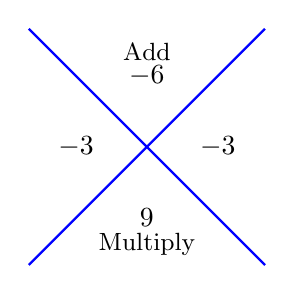
\begin{tikzpicture}[scale=1.5, auto, >=stealth]
				\draw[thick, blue] (-1, 1) -- (1, -1);
				\draw[thick, blue] (-1, -1) -- (1, 1);
				\node at (0, 0.6) {$-6$};
				\node at (0, -0.6) {$9$};
				\node at (-0.6, 0) {$-3$};
				\node at (0.6, 0) {$-3$};
				\node at (0, 0.6) [above=2pt] {\small Add};
				\node at (0, -0.6) [below=2pt] {\small Multiply};
			\end{tikzpicture}
		\end{center}
		$(u - 3) (u - 3) = 0$ \\
		$(u - 3)^2 = 0$ \\
		$(u - 3)  = 0$ \\
		$u = 3 \to 3x + 4 = 3 \to 3x + 4 = 3$ \\
		$3x = -1$ \\
		$x = -\frac{1}{3}$
		\item $f(x) = 3x^4 - 2x^2 - 1$ \\
		$3x^4 - 2x^2 - 1 = 0$ \\
		$3(x^2)^2 - 2(x^2) - 1 = 0$ \\
		$u = x^2$ \\
		$3u^2 - 2u - 1 = 0$ \\
		\begin{center}
			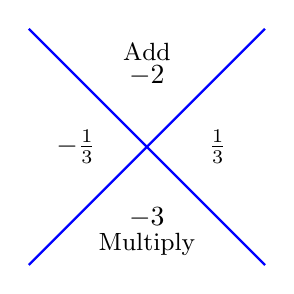
\begin{tikzpicture}[scale=1.5, auto, >=stealth]
				\draw[thick, blue] (-1, 1) -- (1, -1);
				\draw[thick, blue] (-1, -1) -- (1, 1);
				\node at (0, 0.6) {$-2$};
				\node at (0, -0.6) {$-3$};
				\node at (-0.6, 0) {$-\frac{1}{3}$};
				\node at (0.6, 0) {$\frac{1}{3}$};
				\node at (0, 0.6) [above=2pt] {\small Add};
				\node at (0, -0.6) [below=2pt] {\small Multiply};
			\end{tikzpicture}
		\end{center}
		$u = 1 \land u = -\frac{1}{3}$ \\
		$(u - 1)(3u + 1) = 0$ \\
		$u - 1 = 0 \land 3u + 1 = 0$ \\
		$x^2 = 1 \land x^2 = -\frac{1}{3}$ \\
		$\sqrt{x^2} = \pm \sqrt{1} \land \sqrt{x^2} = \pm \sqrt{-\frac{1}{3}}$ \\
		$(x = 1 \land = x = i\sqrt{\frac{1}{3}}) \land (x = -1 \land = x = -i\sqrt{\frac{1}{3}})$
		\item $f(x) = x^\frac{2}{3} - 7x^\frac{1}{3} + 10$ \\
		$x^\frac{2}{3} - 7x^\frac{1}{3} + 10 = 0$ \\
		$(x^\frac{1}{3})^2 - 7(x^\frac{1}{3}) + 10 = 0$ \\
		$u = x^\frac{1}{3}$ \\
		$u^2 - 7u + 10 = 0$ \\
		\begin{center}
			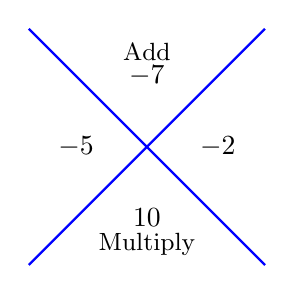
\begin{tikzpicture}[scale=1.5, auto, >=stealth]
				\draw[thick, blue] (-1, 1) -- (1, -1);
				\draw[thick, blue] (-1, -1) -- (1, 1);
				\node at (0, 0.6) {$-7$};
				\node at (0, -0.6) {$10$};
				\node at (-0.6, 0) {$-5$};
				\node at (0.6, 0) {$-2$};
				\node at (0, 0.6) [above=2pt] {\small Add};
				\node at (0, -0.6) [below=2pt] {\small Multiply};
			\end{tikzpicture}
		\end{center}
		$(u - 5) (u - 2) = 0$ \\
		$u - 5 = 0 \land u - 2 = 0$ \\
		$u = 5 \land u = 2$ \\
		$x^\frac{1}{3} = 5 \land x^\frac{1}{3} = 2$ \\
		\textbf{Note: }We can do two methods here. \\
		$\sqrt[3]{x} = 5$ \\
		$(\sqrt[3]{x})^3 = (5)^3$ \\
		$x = 125$ \\
		$x^\frac{1}{3} = 2$ \\
		$(x^\frac{1}{3})^3 = (2)^3$ \\
		$x = 8$
		\item $g(x) = x + \sqrt{x} - 20$ \\
		$x + \sqrt[1]{x^2} - 20 = 0$ \\
		$x^1 + x^\frac{1}{2} - 20 = 0$ \\
		$(x^\frac{1}{2})^2 + (x^\frac{1}{2}) - 20 = 0$ \\
		$u = x^\frac{1}{2}$ \\
		$u^2 + u - 20 = 0$ \\
		\begin{center}
			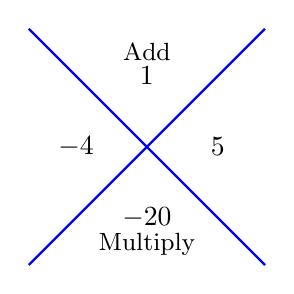
\begin{tikzpicture}[scale=1.5, auto, >=stealth]
				\draw[thick, blue] (-1, 1) -- (1, -1);
				\draw[thick, blue] (-1, -1) -- (1, 1);
				\node at (0, 0.6) {$1$};
				\node at (0, -0.6) {$-20$};
				\node at (-0.6, 0) {$-4$};
				\node at (0.6, 0) {$5$};
				\node at (0, 0.6) [above=2pt] {\small Add};
				\node at (0, -0.6) [below=2pt] {\small Multiply};
			\end{tikzpicture}
		\end{center}
		$u = 4 \land u = -5$ \\
		$x^\frac{1}{2} = 4 \land x^\frac{1}{2} = -5$ \\
		$\sqrt{x} = 4 \land \sqrt{x} = -5$ \\
		$(\sqrt{x})^2 = (4)^2 \land (\sqrt{x})^2 = (-5)^2$ \\
		$x = 16 \land x = 25$ \\
		\textbf{Note: }$x = 25$ is not a real solution because a square root can't equal a negative.
		\item $h(x) = -2y^{-2} - 11y^{-1} + 40$ \\
		$-2y^{-2} - 11y^{-1} + 40 = 0$ \\
		$2y^{-2} + 11y^{-1} - 40 = 0$ \\
		$2(y^{-1})^2 + 11 (y^{-1}) - 40 = 0$ \\
		$u = y^{-1}$ \\
		$2u^2 + 11u - 40 = 0$ \\
		\begin{center}
			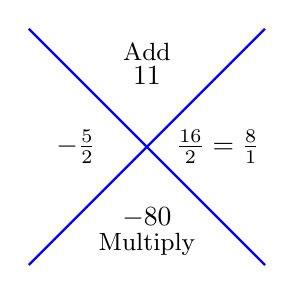
\begin{tikzpicture}[scale=1.5, auto, >=stealth]
				\draw[thick, blue] (-1, 1) -- (1, -1);
				\draw[thick, blue] (-1, -1) -- (1, 1);
				\node at (0, 0.6) {$11$};
				\node at (0, -0.6) {$-80$};
				\node at (-0.6, 0) {$-\frac{5}{2}$};
				\node at (0.6, 0) {$\frac{16}{2} = \frac{8}{1}$};
				\node at (0, 0.6) [above=2pt] {\small Add};
				\node at (0, -0.6) [below=2pt] {\small Multiply};
			\end{tikzpicture}
		\end{center}
		$(2u - 5) (u + 8) = 0$ \\
		$2u - 5 = 0 \land u + 8 = 0$ \\
		$u = \frac{5}{2} \land u = -8$ \\
		$y^{-1} = \frac{5}{2} \land y^{-1} = -8$ \\
		$\frac{1}{y} = \frac{5}{2} \land \frac{1}{y} = -8$ \\
		$y = \frac{2}{5} y = -\frac{1}{8}$
	\end{enumerate}
\end{example}
